\chapter{Domainmodell}

\section{Architekturmodell}
	Der logische Aufbau der Software besteht aus vier Schichten:
	\begin{figure}[h]
		\centering
		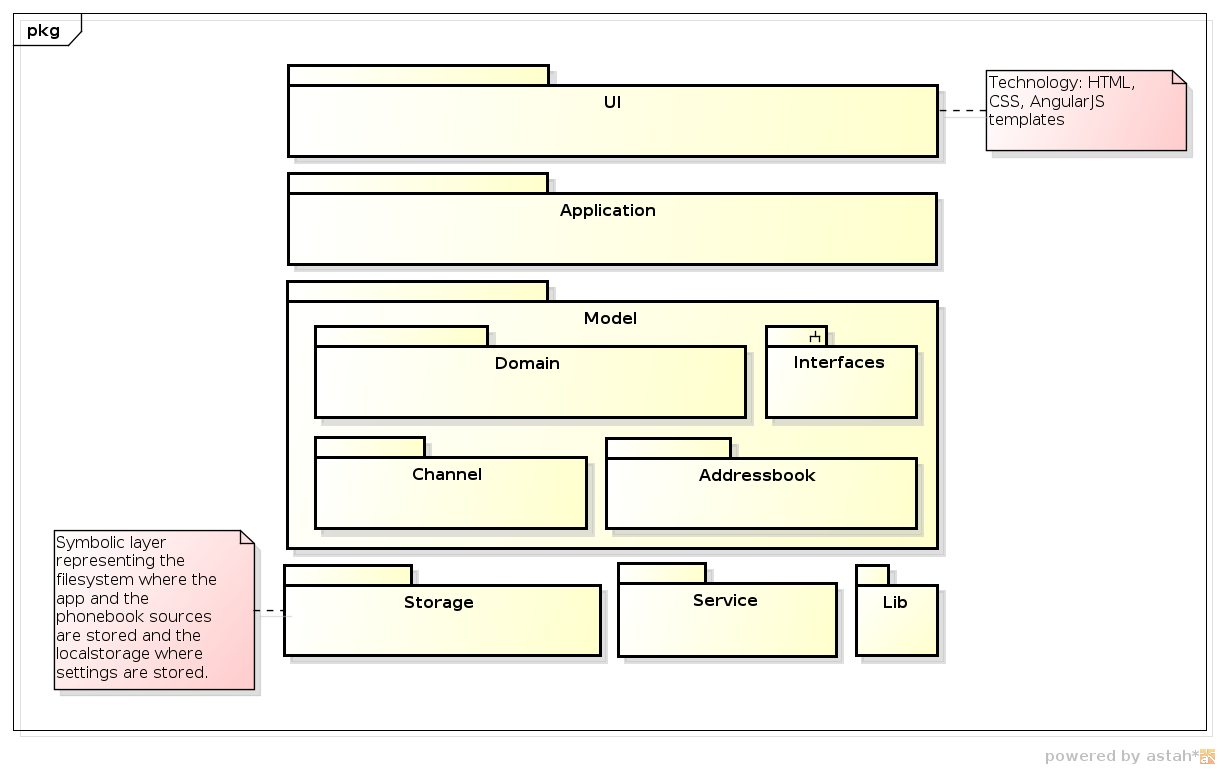
\includegraphics[width=1\textwidth]{../architekturanalayse/img/architecture.png}
		\caption{Architekturdiagramm JS VoIP App}
	\end{figure}

	\begin{landscape}
		\section{Strukturdiagramm}
			Im folgenden Diagramm sind die wichtigsten konzeptionellen Klassen und ihre Beziehungen untereinander aufgeführt.
			\begin{figure}[h]
				\centering
				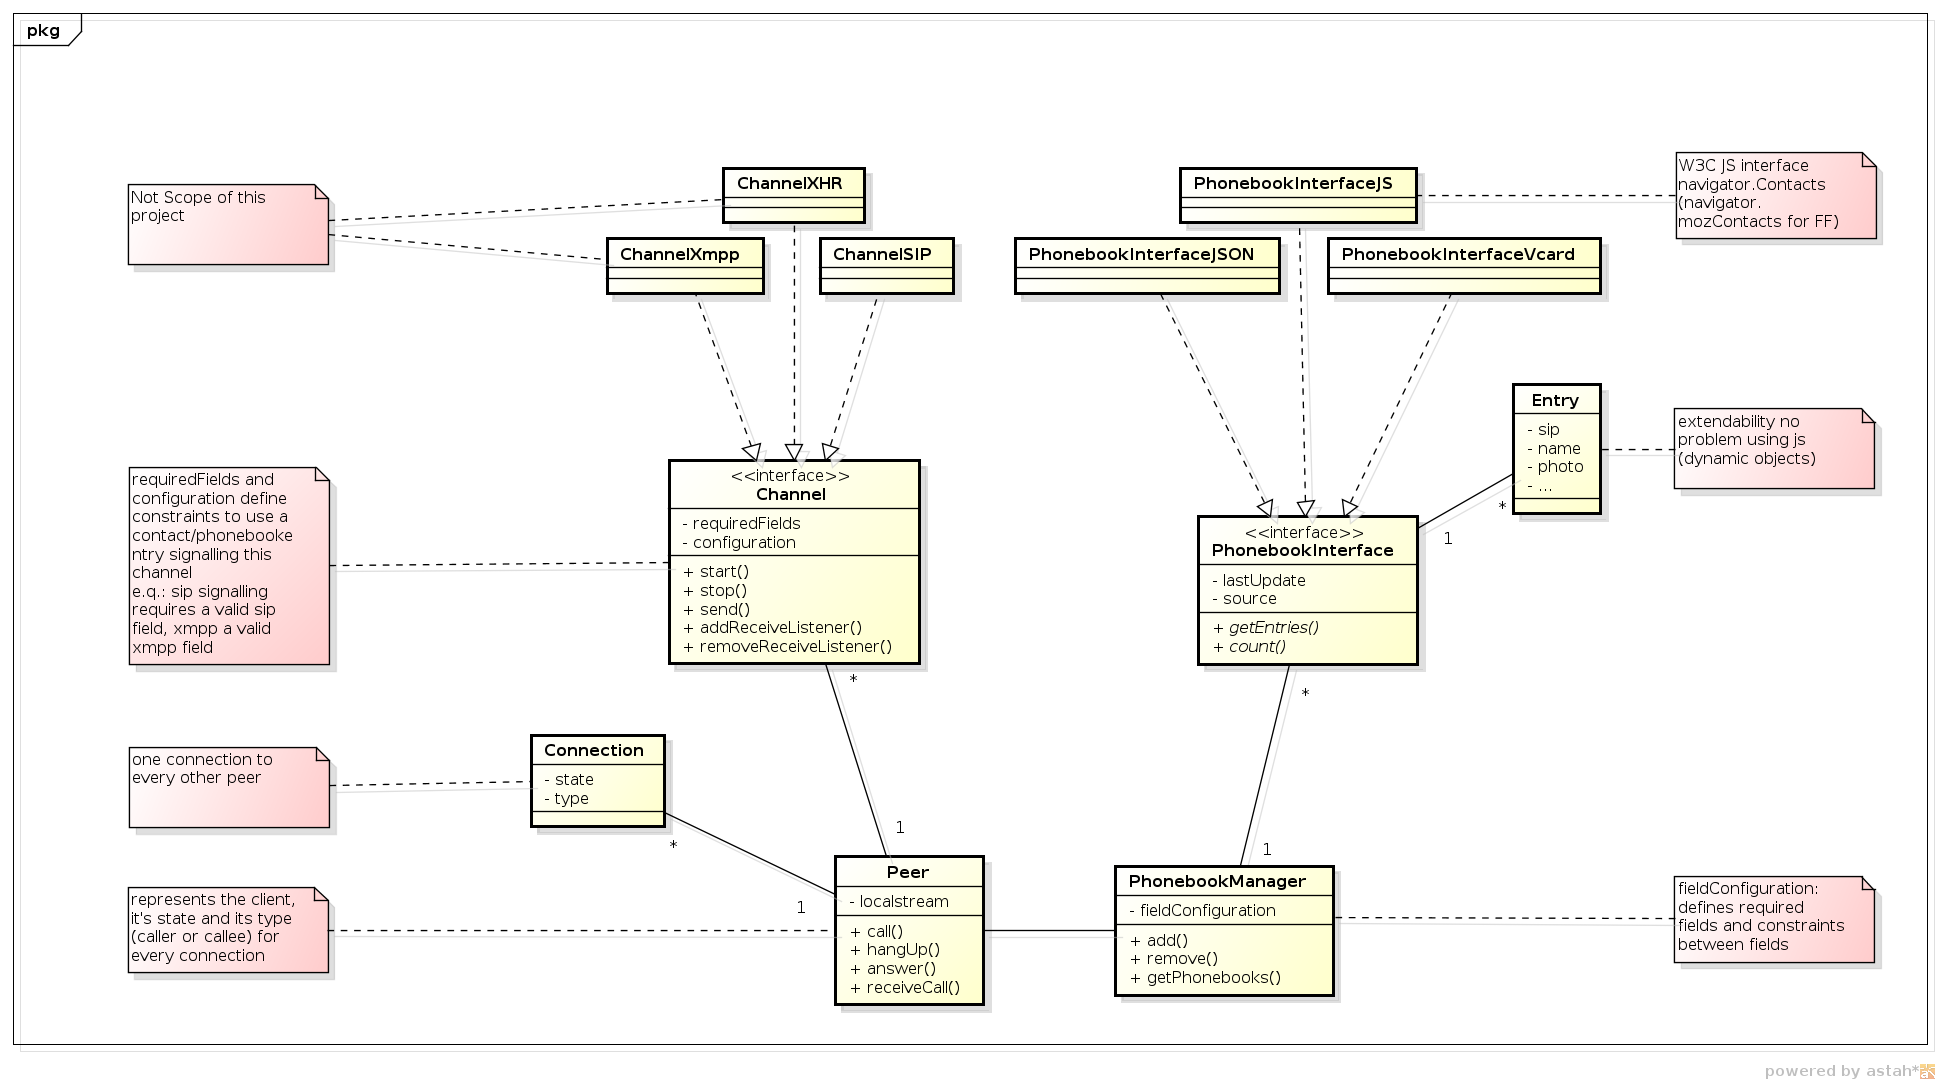
\includegraphics[width=1.2\textwidth]{../architekturanalayse/img/domain.png}
				\caption{Strukturdiagramm JS VoIP App}
			\end{figure}
	\end{landscape}
	\clearpage

\section{Architektur Designmotivations}
	\subsection{Client/Server vs. reine Client Applikation}
		\subsubsection{Vorteile Client-/Server Umsetzung}
		\begin{itemize}
			\item Schlanker Client
			\item Es wird nur eine Schnittstelle benötigt zwischen Client und Server, der gesammte Verkehr kann über HTTP abgewickelt werden.
			\item Nur der Server muss die Schnittstellen zu andern Diensten unterstützen. Keine zusätzlichen Schnittstellenanforderungen an den Client
			\item Es ist einfacher durch Firewalls durchzukommen, da die Kommunikation genau kontrolliert werden kann.
		\end{itemize}
		\subsubsection{Nachteile}
		\begin{itemize}
			\item Redundanzen, da Funktionalität zwischen dem Client und Server durch ein eigene Protokoll erneut übersetzt wird und damit auf beiden Seiten Teile der gleichen Funktionalität umgesetzt werden müssen.
			\item Ein Anwender ist an den Server, bzw. diese Serverimplementation gebunden. Die Applikation läuft nicht ohne den Server.
			\item Server ist ``Single Point of Failure''
			\item Sollen weitere Schnittstellen umgesetzt werden, so muss der Server erweitert werden, was aufwendiger ist als den Client zu erweitern
		\end{itemize}


		\subsubsection{Vorteile reine Client Lösung}
		\begin{itemize}
			\item Es wird kein Server benötigt
			\item Anwender können einen beliebigen Kommunikationsserver (SIP\footnote{Session Initiation Protocol}) verwenden, bzw. sogar eine eigene Channelimplementation hinzufügen um z.B. über XMPP\footnote{Extensible Messaging and Presence Protocol} das Signalling durchzuführen
			\item Um die Applikation für weitere Schnittstellen zu erweitern sind keine Kenntnisse der Servertechnologie notwendig
			\item Die Applikation insgesammt ist weniger aufwändig aufgebaut weil sie weniger Redundanzen beinhaltet
			\item Keine eigene SIP / XMPP Server Implementation (Es braucht nur bereits vorhandene Serverinfrastrukturen)
		\end{itemize}
		\subsubsection{Nachteile}
		\begin{itemize}
			\item Die möglichen Schnittstellen sind auf Browserfunktionalität begrenzt (HTTP, WebSockets, RTSP\footnote{Realtime Strem Protocol}). Dadurch muss ein SIP oder XMPP Provider WebSockets unterstützen, damit er für das Signalling benutzt werden kann.
			\item Der Client wird etwas umfangreicher
			\item Probleme mit Firewalls und Router möglich, die WebSocket Pakete nicht weiterleiten. WebSockets können grundsätzlich über einen beliebigen Port laufen, meisst wird jedoch Port 80 verwendet. Trotzdem leiten einige Router die Pakete nicht weiter.
			\item Performanceprobleme möglich, da sämmtliche Logik inklusive dem Parsen der verschiedenen Protokolle vom Client abgearbeitet werden muss.
		\end{itemize}

		\subsubsection{Fazit}
			Aufgrund geringerer Abhängigkeiten und der Wahrscheinlichkeit, das SIP Server Provider irgendwann WebSockets unterstützen, wird die Lösung ``reine Client Applikation'' gewählt.
			Für die Kommunikation mit Signallingservern wie SIP oder XMPP werden WebSockets eingesetzt, für Signalling über XHR\footnote{XmlHTTPRequest} wird mit der Option ``Allow Cross Origin'' gearbeitet.

	\subsection{STUN Service}
		STUN\footnote{Session Traversal Utilities for NAT} Services sind zwingend notwendig um die nach aussen sichtbare IP Adresse des Clients herauszufinden. Nebst der Möglichkeit selbst einen STUN Service aufzusetzen, gibt es frei verfügbare STUN Services, z.B. von Mozilla oder Google.

		Für ein Abgeschottetes Netz ist ein eigener STUN Server zwingend notwendig. Für unsern Fall reichen die frei verfügbaren. Durch anpassen der Konfiguration ist es möglich den Server festzulegen.

		Im Netz gibt es fertig konfigurierte Virtuelle Maschinen mit einsatzbereitem STUN-Service\footnote{Mozilla, stun-vm (Stand: 15.01.13). \hyperlink{https://github.com/mozilla/stun-vm}{https://github.com/mozilla/stun-vm} [Abgerufen am 28.10.13]}.

	\subsection{SIP Proxy vs. SIP Server mit WebSockets}
		Unterstützt ein SIP Server keine WebSockets, so kann ein SIP/WebSocket Proxy dazwischen geschaltet werden. Die Konfiguration eines SIP Proxies ist ähnlich aufwändig wie die Installation eines Kamailio\footnote{Kamailio SIP Server Project, Features (Stand: 18.03.2013). \hyperlink{http://www.kamailio.org/w/features/}{http://www.kamailio.org/w/features/}, [Abruf am 28.10.13]} SIP Servers, der in der neusten Version WebSockets unterstützt.

		Aus diesem Grund wird ein eigener SIP Server dem Proxy vorgezogen.

	\subsection{Sicherheit}
		WebRTC Streams können nur verschlüsselt übertragen werden. Es gibt keine Möglichkeit die Verschlüsselung abzuschalten. Dies führt zwar zu einem erhöhten Rechenbedarf auf dem Client, garantiert jedoch eine verschlüsselte Verbindung unabhängig den Vorlieben des Entwicklers.
		Die Verschlüsselung erfolg über DTLS-SRTP\footnote{IETF, RFC5764 (Stand: 2010). \hyperlink{http://tools.ietf.org/html/rfc5764}{tools.ietf.org/html/rfc5764}, [Abruf am 28.10.13]} keyings\footnote{Adam Roach, WebRTC: Security and Confidentiality (Stand: 07.06.13). \hyperlink{http://sporadicdispatches.blogspot.ch/2013/06/webrtc-security-and-confidentiality.html}{http://sporadicdispatches.blogspot.ch/2013/06/webrtc-security-and-confidentiality.html}, [Abruf am 28.10.13]}. 
		
		Die Verschlüsselung des Signalling Channels ist abhängig von der eingesetzten Technologie. Werden z.B. Secure Websockets oder XHR über HTTPS eingesetzt so ist die Kommunikation verschlüsselt und nicht abgreifbar.
		
		Trotzdem kann ein Provider oder ein Geheimdienst Metadaten darüber sammeln, wer mit wem telefoniert.
		  
	\subsection{Hosting}
		Die JS VoIP App kann sowohl lokal ausgeführt werden wie von einem Webserver ausgeliefert ausgeführt werden. Es gibt keine speziellen Voraussetzungen. Ein Webserver ist daher nicht zwingend notwendig.
	
\clearpage
\section{Deployment}
	\begin{figure}[h]
		\centering
		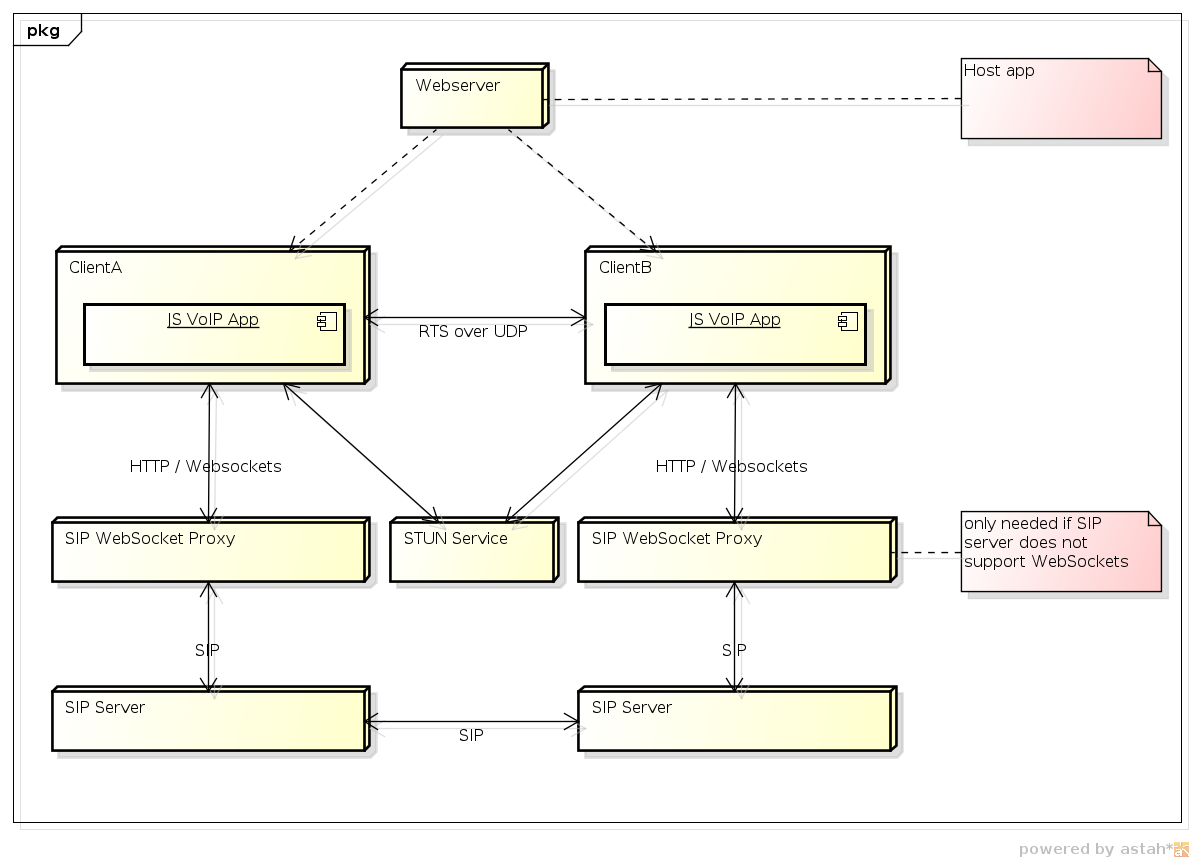
\includegraphics[height=0.7\textwidth]{../architekturanalayse/img/deployment.png}
		\label{img:deployment}
		\caption{Deploymentdiagramm JS VoIP App}
	\end{figure}
	